\documentclass[12pt]{article}
\usepackage[utf8]{inputenc}
\usepackage[brazil]{babel}
\usepackage{hyphenat}
\usepackage{graphicx}
\usepackage{amsmath}
\graphicspath{{images/}}
\usepackage{float}
\usepackage{listings}

% ---- Capa
\title{%
    Modelagem de Sistemas Dinâmicos\\
    \large Trabalho 5}
\author{Erica da Cunha Ferreira}
\date{Novembro 2020}
\begin{document}
\maketitle
\pagenumbering{gobble}
\vspace{8cm} %5mm vertical space
\begin{center}
    
\includegraphics[width=0.2\textwidth]{logo.png}
\end{center}

%-----Sumário
\newpage
\tableofcontents
\newpage
\pagenumbering{gobble}

%----Pág 1
\cleardoublepage\pagenumbering{arabic}

\section{Resumo}

\quad Neste trabalho temos os sinais de entrada $u(t)$ e de saída $y(t)$ de um sistema linear contínuo $G(s)$. Sendo que os sinais $u$ e $y$ foram aplicados e aquistados com uma frequência de amostragem $f_s = 2Hz$ ( período de amostragem $T = 0.5s$). Sendo $t$ o vetor de tempo discreto.

\section{Introdução}

\quad Este trabalho tem como objetivo analisar os aspectos de entrada de resposta em frequência, uma vez que foram dados dois sinais de um sistema linear contínuo,$u(t)$ e $y(t)$, de entrada e saída, respectivamente. Para esta análise, é importante salientar que o sinal está  com ruído. 

\section{Metodologia}
\subsection{Sinal de Entrada}
\quad O código abaixo foi escrito utilizando o software Matlab, a partir dele é determinado o módulo, fase e o espectro de sinal da entrada da função de transferência em $Hz$.

\begin{lstlisting}[language = Matlab]

    Y = fft(y);
    U = fft (u);
    Fs = 2;
    N = length (u);
    f = [0:N-1]*Fs/N;
    G = Y./U;

    figure(1)
    subplot(2,1,1)
    plot(f,20*log10(fftshift(abs(U))));
    xlabel('Hz'); ylabel('dB');
    subplot(2,1,2)
    plot(f,rad2deg(angle(U)));
    xlabel('Hz'); 
\end{lstlisting}
\quad Algoritmo feito no Matlab.\\

\quad A partir dos dados obtidos utizando o código acima, foi possível plotar o gráfico abaixo:

\begin{figure}[H] 
    \centering
    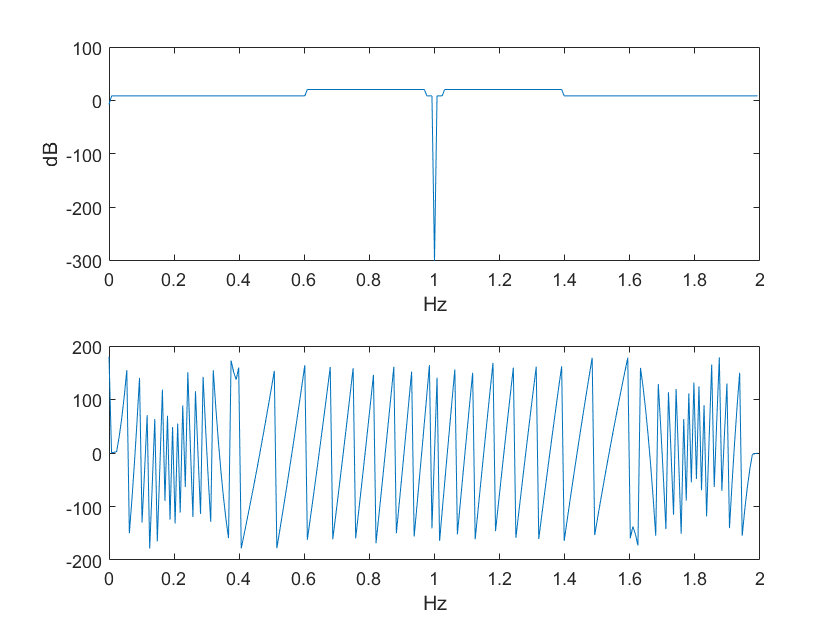
\includegraphics[width=0.7\textwidth]{Gráfico01.png}
    \caption{Espectro do sinal de entrada.}
    \label{fig:mesh2}
\end{figure}

\quad No gráfico da Figura(1) na parte superior, podemos observar a resposta do módulo com a frequência. Nele, temos um pico, este indica a frequência de uma senoide. Como foi indicado na Figura(2), abaixo, essa característica está presente quando se é analisada os sinais cossenoidais.

\begin{figure}[H] 
    \centering
    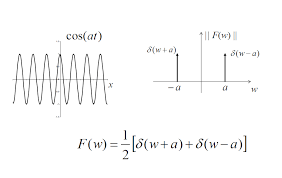
\includegraphics[width=0.5\textwidth]{funçãocos.png}
    \caption{FTT de sinal cossenoidal}
    \label{fig:mesh2}
\end{figure}

\par Como é possível perceber na comparação entre as figuras acima, o impulso da Figura(1) é invertido em relação ao eixo x, das abscissas. Isto se deve ao fato do sinal esperado da função que aparenta ser negativo.

\subsection{Resposta em Frequência}
\quad A partir do algoritmo abaixo, foi possível encontrar a resposta em frequência do sistema em análise:

\begin{lstlisting}[language = Matlab]

    Y = fft(y);
    U = fft (u);
    Fs = 2;
    N = length (u);
    f = [0:N-1]*Fs/N;
    G = Y./U;

    figure(1)
    subplot(2,1,1)
    plot(f,20*log10(fftshift(abs(G))));
    xlabel('Hz'); ylabel('dB');
    subplot(2,1,2)
    plot(f,rad2deg(angle(G)));
    xlabel('Hz'); 
\end{lstlisting}


\quad Como resultado, obtemos os gráficos:

\begin{figure}[H] 
    \centering
    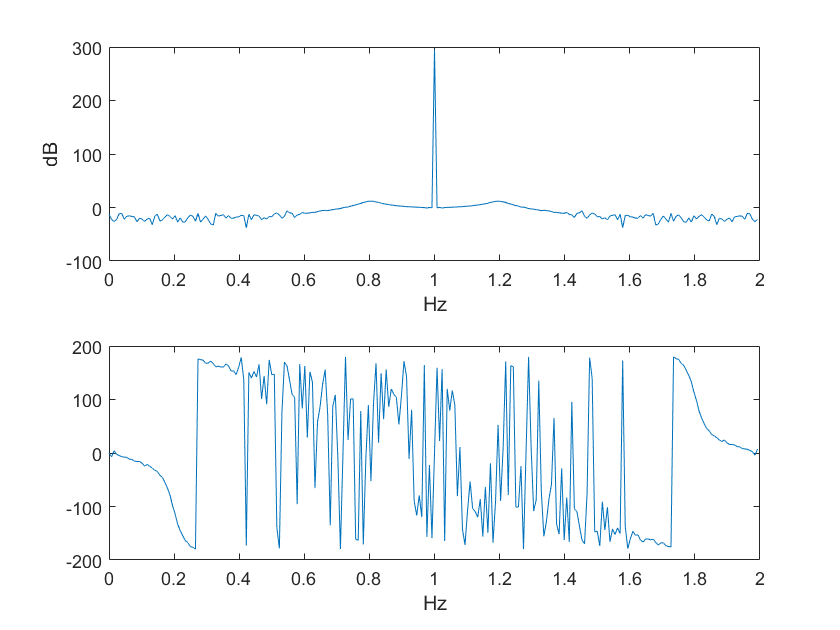
\includegraphics[width=0.7\textwidth]{Gráfico 02.png}
    \caption{Espectro da resposta em frequência.}
    \label{fig:mesh2}
\end{figure}
\par Com o uso da funcionalidade "System Identification Toolbox" do Matlab, é possível representar matematicamente a função de transferência, dadas as entrada e saída. Ao selecionar "Transfer Function Model" e colocando o uso de dois polos e zeros, é obtido a seguinte forma fechada:

\begin{equation}
    G(s) = \frac{0.3053s^2 - 0.1155s + 0.06864}{s^2 + 0.04855s + 0.6439}
\end{equation}

\section{Conclusão}
\quad Ao analisar o Figura(3) e das outras respostas obtida pelas simulações, vemos que este se trata de um filtro passa banda, isto é, as frequências longe do pico  são descartadas, enquanto as mais próximas do pico passam. Vale reafirmar que o gráfico contém ruídos.

\end{document}
